\documentclass[tikz,border=2pt,11pt]{standalone}
\usetikzlibrary{arrows.meta}
\usepackage{amsmath}
\usepackage{amssymb}
\usepackage{xcolor}
\usepackage{tikz}
\newcommand{\C}{\mathbb C}
\newcommand{\R}{\mathbb R}
\newcommand{\N}{\mathbb N}
\newcommand{\Z}{\mathbb Z}
\newcommand{\B}{\mathcal B}
\DeclareMathOperator{\BC}{BC}
\DeclareMathOperator{\id}{id}
\DeclareMathOperator{\supp}{supp}
\DeclareMathOperator{\Aut}{Aut}
\DeclareMathOperator{\Dom}{Dom}
\DeclareMathOperator{\linspan}{span}
\begin{document}
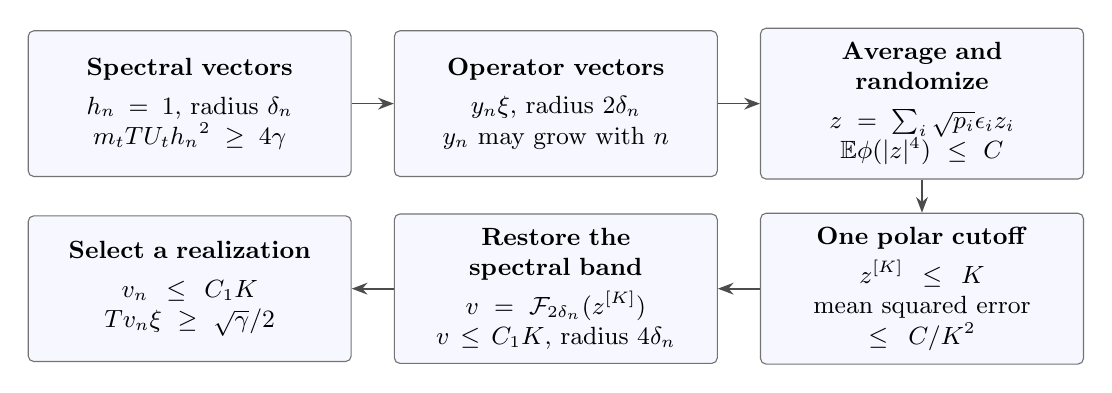
\begin{tikzpicture}[
  stage/.style={draw=black!55,rounded corners=2pt,fill=blue!3,
    text width=3.75cm,minimum height=1.85cm,align=center,
    inner sep=5pt,font=\small},
  flow/.style={-{Stealth[length=2mm]},semithick,draw=black!70}]
  \node[stage] (input) at (0,0) {
    \textbf{Spectral vectors}\\[3pt]
    $\norm{h_n}=1$, radius $\delta_n$\\
    $m_t\norm{TU_th_n}^2\ge4\gamma$};
  \node[stage] (approx) at (4.65,0) {
    \textbf{Operator vectors}\\[3pt]
    $y_n\xi$, radius $2\delta_n$\\
    $\norm{y_n}$ may grow with $n$};
  \node[stage] (random) at (9.3,0) {
    \textbf{Average and randomize}\\[3pt]
    $z=\sum_i\sqrt{p_i}\epsilon_i z_i$\\
    $\mathbb E\phi(|z|^4)\le C$};
  \node[stage] (cutoff) at (9.3,-2.35) {
    \textbf{One polar cutoff}\\[3pt]
    $\norm{z^{[K]}}\le K$\\
    mean squared error\\
    $\le C/K^2$};
  \node[stage] (filter) at (4.65,-2.35) {
    \textbf{Restore the spectral band}\\[3pt]
    $v=\mathcal F_{2\delta_n}(z^{[K]})$\\
    $\norm{v}\le C_1K$, radius $4\delta_n$};
  \node[stage] (output) at (0,-2.35) {
    \textbf{Select a realization}\\[3pt]
    $\norm{v_n}\le C_1K$\\
    $\norm{Tv_n\xi}\ge\sqrt\gamma/2$};
  \draw[flow] (input) -- (approx);
  \draw[flow] (approx) -- (random);
  \draw[flow] (random) -- (cutoff);
  \draw[flow] (cutoff) -- (filter);
  \draw[flow] (filter) -- (output);
\end{tikzpicture}
\end{document}
